\section{Cours 5}
\subsection{Beyond flows}
\begin{figure}[!ht]
	\subsubsection{MAX-SAT comme PL(en nombre entiers)}
	\textbf{Entrée:} Une formule booléenne f=c$_1\wedge$...$\wedge$c$_m$ en forme normale conjective avec n
	variables x$_1$, ..., x$_n$.\\
	\textbf{Sortie:} Une affectation 0-1 des variables dont le poids total des clauses satisfaites soit max.\\
	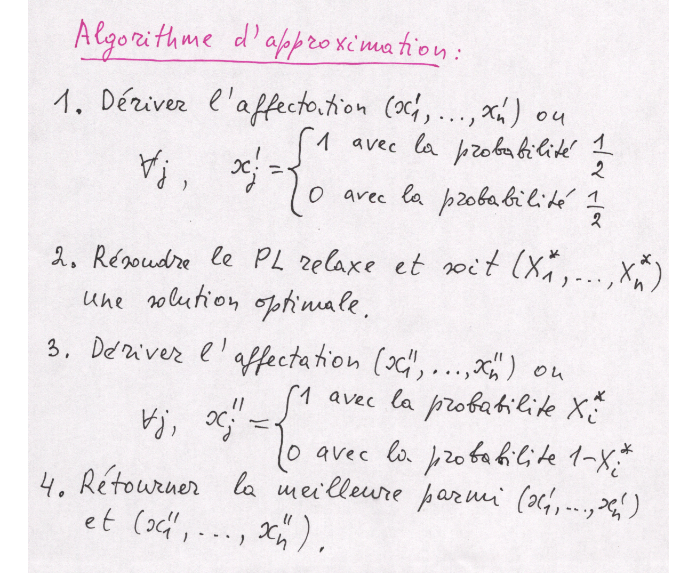
\includegraphics[width=\linewidth,height=0.75\textheight]{notes/algorithme/algo_appro.png}
	\textbf{Théorème:\\}
	Le poids espéré des clauses satisfaites par l'affectation de l'algorithme est $\geq\frac{3}{4}$ poids optimal.
	Donc, l'algo est un algorithme d'approximation facteur $\frac{3}{4}$.
\end{figure}
\begin{figure}[!ht]
	\subsubsection{Couverture de sommets}
	\textbf{Entrée:} Un graphe G=(V,E) où chaque sommet v$\in$V a un poids positif w$_v>$0.\\
	Une couverture de sommet est un sous ensemble S$\subset$V tel que, $\forall$ arrête uv de G,
	\{u,v\}$\cap$S$\neq$0. Le poids de S est w(S)=$\Sigma_{v \in S}w_v$.\\
	\textbf{But:} Trouver une couverture de poids minimal de G.\\
	\textbf{Difficulté:} NP-complet déjà dans le cas non pondéré (w$_v$=1, $\forall$v$\in$V).\\
	\textbf{Lemme:\\}
	Les solutions admissibles de PLNE sont en bijection avec les couvertures de sommets de G.\\
	\textbf{Théorème:\\}
	S=\{v$\in$V: x$_v^+$=1\} est une couverture de sommet de G. De plus, w(S)$\leq$2OPT.
\end{figure}
